% Chapter 4

\chapter{后端设计}

\section{概述}

本系统的后端整体上是基于Spring Boot框架开发起来的,代码用Java编写。图\ref{fig:package}是以包为单位绘制的,一个简要的后端代码结构关系图。

\begin{figure}[!htb]
	\centering
	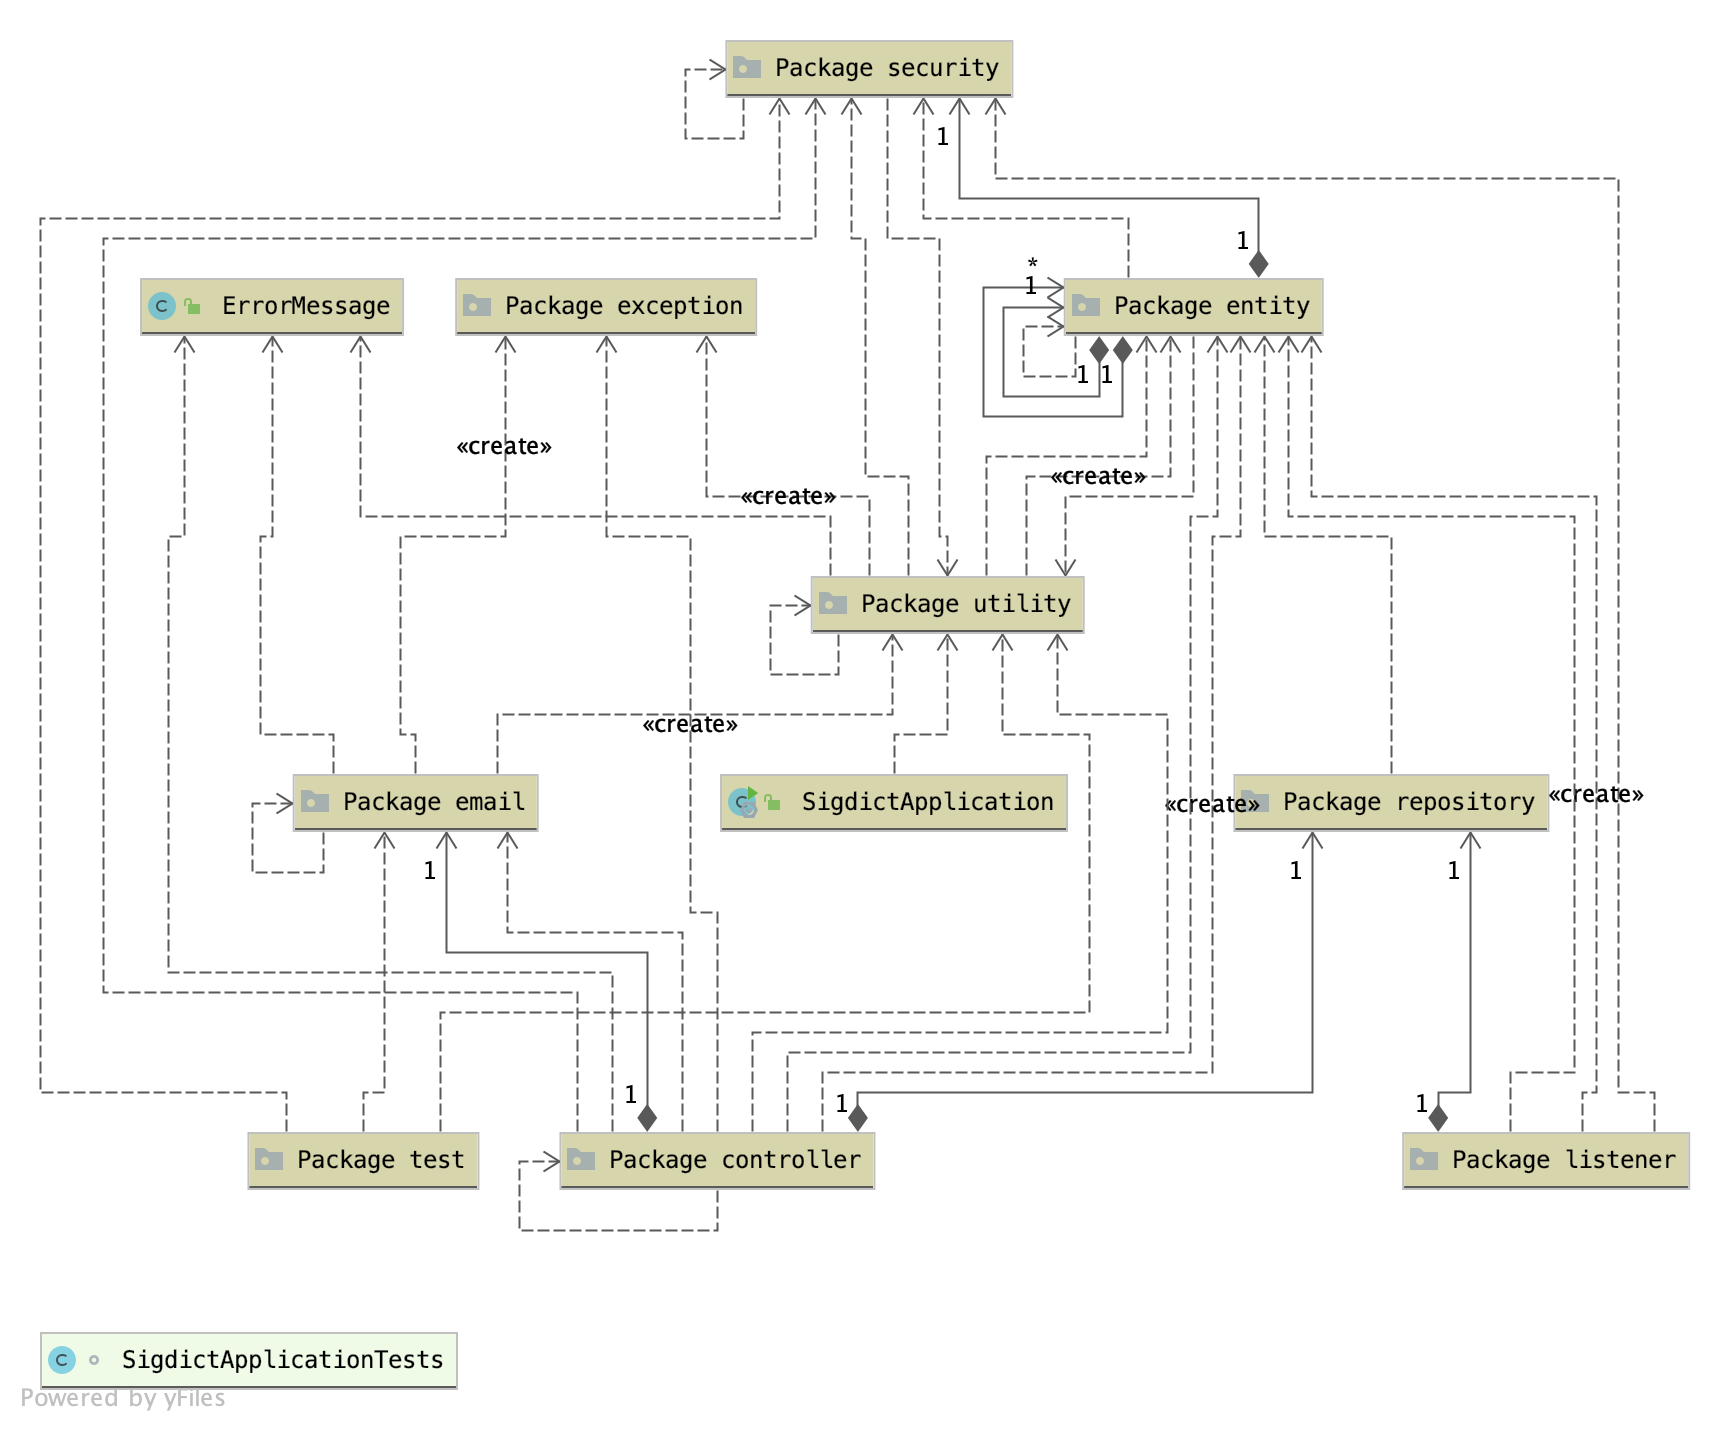
\includegraphics[width=0.8\textwidth]
	{figures/package.png}\\
	\caption{后端Java代码的关系图}
	\label{fig:package}
\end{figure}

\begin{itemize}

	\item \textbf{Package email}
	
	包含了有关发送电子邮件的代码,详见小节\ref{sec:emailP}。
	
	\item \textbf{Package controller}
	
	包含了所有Controller类,详见小节\ref{sec:controllerP}。

\end{itemize}

\section{发送电子邮件服务}\label{sec:emailP}

我们将通过JavaMail库的帮助与一个SMTP服务器建立联系,并最终将邮件推送到用户的设备上,相关代码位于包email中。

因为Google提供小规模免费的SMTP服务,我们这里就以Google的SMTP服务为例。为了成功的发送电子邮件,我们首先需要配置相应的SMTP服务器地址和端口,下方代码片段示例的4-5行完成了这项工作。同时往往提供这类服务的服务器需要使用者登录,因此在第10行完成了用用户名、密码登录验证的操作。

\begin{minted}
[
	frame=lines,
	framesep=2mm,
	baselinestretch=1.2,
	bgcolor=lightgray,
	fontsize=\footnotesize,
	linenos
]{java}

Properties props = new Properties();
props.put("mail.smtp.auth", "true");
props.put("mail.smtp.starttls.enable", "true");
props.put("mail.smtp.host", "mail.smtp.host");
props.put("mail.smtp.port", "587");

Session session = Session.getInstance(props,
        new javax.mail.Authenticator() {
                protected PasswordAuthentication getPasswordAuthentication() {
                        return new PasswordAuthentication(username, password);
                }
        }
);

\end{minted}

这之后只需要如下代码片段所示,将邮件的收件人地址、主体、正文等信息设置妥当后,就可以执行发送的命令,送出这份电子邮件。我们所选择的SMTP服务器在收到这封电子邮件后,将会尝试将它推送给接收用户所属的SMTP服务器。在推送成功后,接收用户便可以从所属的SMTP服务器中拉取、查看这封电子邮件。

\begin{minted}
[
	frame=lines,
	framesep=2mm,
	baselinestretch=1.2,
	bgcolor=lightgray,
	fontsize=\footnotesize,
	linenos
]{java}

Message message = new MimeMessage(session);
message.setFrom(new InternetAddress(fromEmail));
message.setRecipients(Message.RecipientType.TO, InternetAddress.parse(toEmail));
message.setSubject(subject);
message.setText(content);
Transport.send(message);

\end{minted}

发送电子邮件因为涉及网络IO交互,所以相比于其他操作会产生巨大的延迟。为了提高响应速度,让用户拥有更好的使用体验,我们利用Spring Boot的@Async关键词对本模块做了一层封装修饰。让发送方式从同步阻塞变成异步非阻塞,增加效率,显著减少了用户需要等待的时间。但这样做有利有弊,缺点是即使服务器端发生错误(如500服务器内部错误),导致电子邮件发送失败,用户也无法得到相应的错误提示,用户会错以为我们已经正确的发送了电子邮件。

\section{用户Session的维护}

用户需要登录后才能进行上传文件、下载文件、查看文件数字签名等操作。因为我们必须在用户登录后在服务器端记录一些信息,用于维持用户的登录状态,在这里我们采用了生成Session的方式维持该状态。

具体而言,用户在成功的登录之后,服务器端会随机的生成一个长度为16字节的二进制数据,并将其转化为base64编码\cite{base64}作为用户的Session。这个Session数据首先会被存储在服务器端数据库中,然后会被通过Cookie\cite{cookie}的方式返还给用户。之后用户每次访问我们网站的时候浏览器都会把这个Cookie发送给服务器端,我们会将之与数据库中的信息进行对比,判断用户所处的状态,并给出不同的响应结果。

关于Session的安全分析详见小节\ref{sec:sessionS}。

\section{Controller}\label{sec:controllerP}

Controller作为一个MVC框架的组成部分在网站的整体响应过程中起着至关重要的作用。表\ref{tab:controller}简要列举了我们设计的所有Controller类。

\begin{table}[ht]
\centering
\begin{tabular}{>{\bfseries}lp{8cm}}
\toprule
SessionController & 
一个抽象类,包含了一些用于验证、管理Session的方法,其他所有需要处理Session的Controller都将继承该类。\\
\midrule
EmailController & 
继承自SessionController,负责处理与电子邮件相关的请求。\\
\bottomrule
\end{tabular}
\caption{Controller类}
\label{tab:controller}
\end{table}
